
\mychapter{Dataset}{Dataset}{}
\label{chap:systemmethods}


The dataset used in this project consists of satellite imagery sourced from Google Earth and covers five waste water treatment works (WWTW) facilities: Atlantis, Cape Flats, Waterval, Fisantekraal and Noordelike werke. Each image is a snapshot of a facility's biological reactors at a particular point in time, with filenames encoding the capture date in a \texttt{month\_year} format.


\begin{figure}[htbp] 
    \centering 
    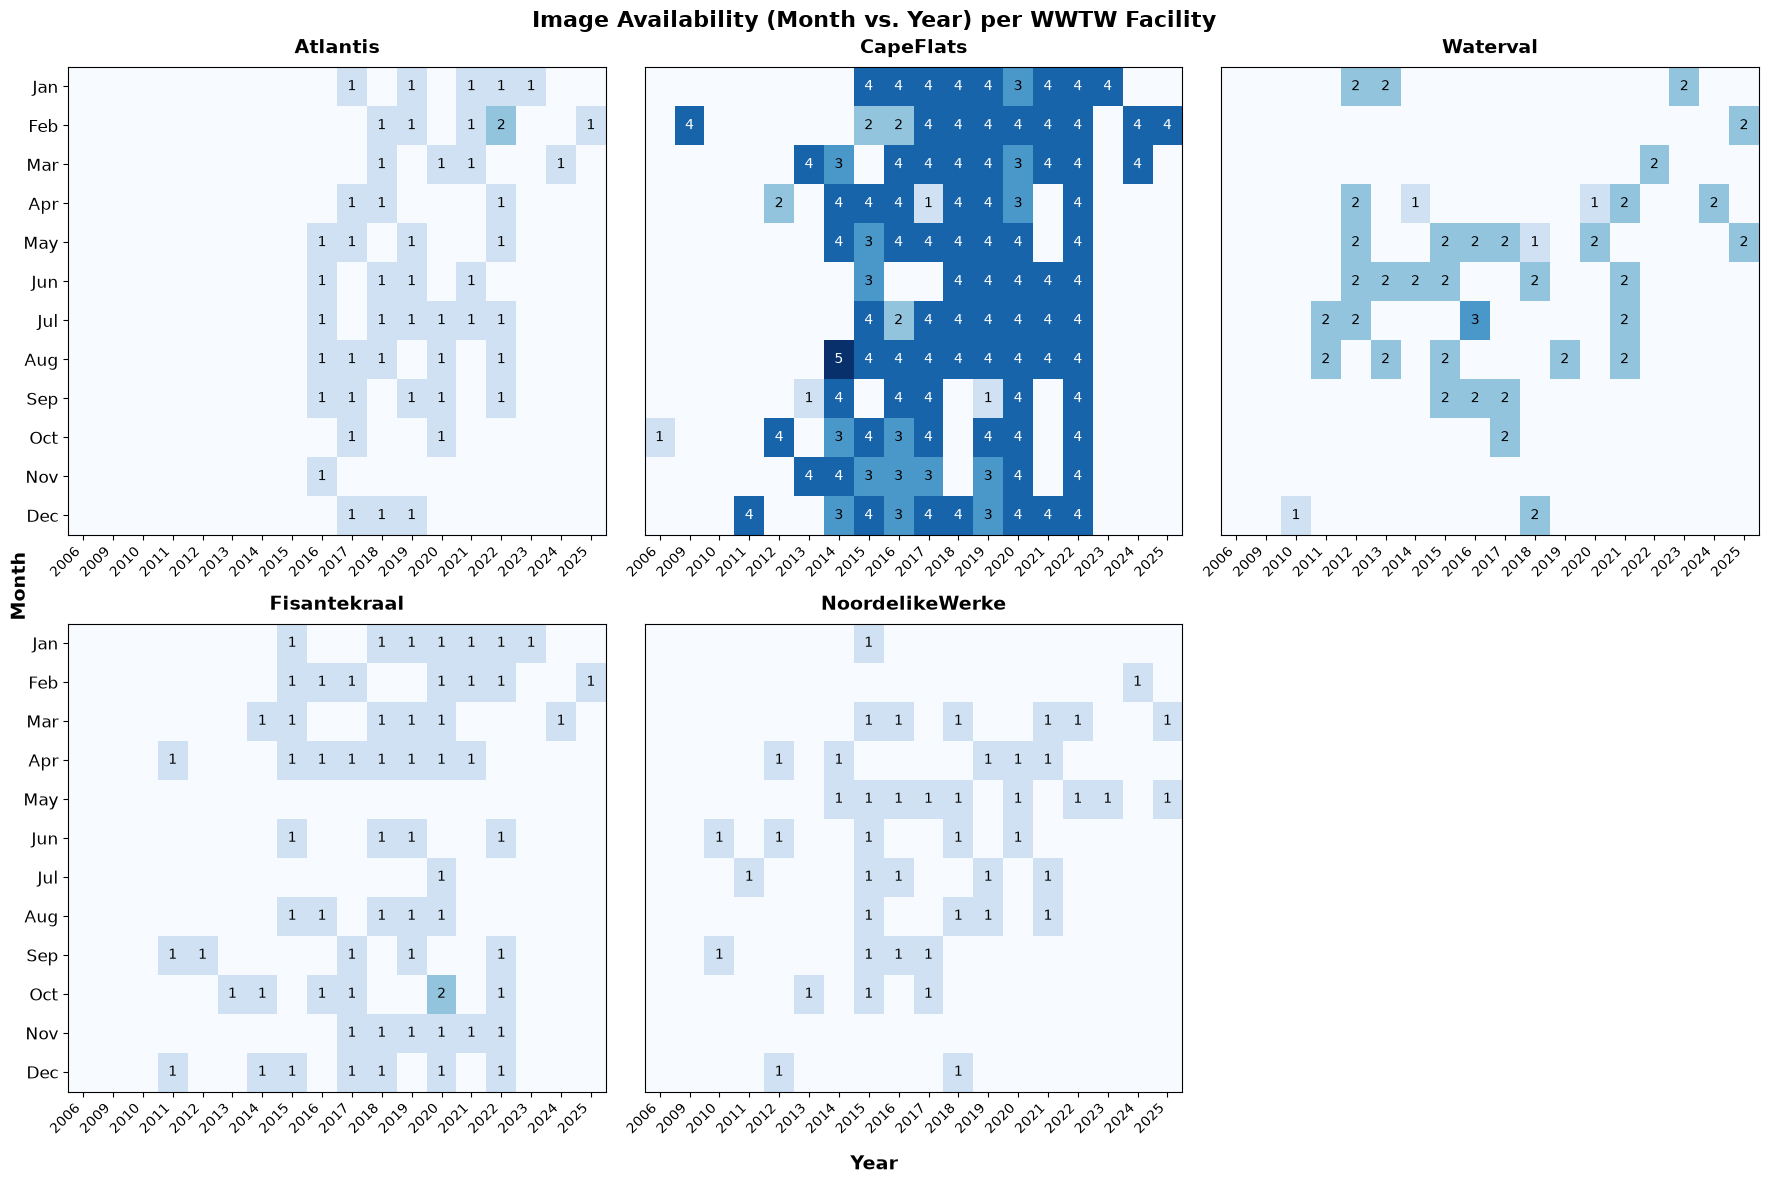
\includegraphics[width=1\textwidth]{figures/heatmap.png} 
    \caption{Distribution of images available in the dataset for each of the five facilities. The numbers indicate how many images are available in the indicated month.}\label{fig:heatmap} 
\end{figure}

As seen in Figure \ref{fig:heatmap}, most images were captured between 2016 and 2022 in the months April to August.

\section{WWTW Sites}

Atlantis WWTW is located on Mission Express Way in Cape Farms, Cape Town. As part of the greater Cape Town municipality, this facility falls within the Western Cape province. Cape Flats WWTW is also situated in the Western Cape; this sewage treatment plant is located on Informal Road in the Southern Suburbs of Cape Town. Additionally, the Western Cape is home to Fisantekraal WWTW, which is situated approximately 10 kilometres north of Durbanville. Waterval WWTW is operated by ERWAT (Ekurhuleni Water Care Company) and is situated in the Gauteng province. Also located in Gauteng is Northern Works (Noordelike Werke) in Johannesburg. It is the largest wastewater treatment plant in Johannesburg and ranks among the largest in South Africa, treating approximately 400 million litres of wastewater every day. The locations of these sites are shown in Figure \ref{fig:map}. An overview of the Atlantis, Cape Flats, Waterval, Fisantekraal, and Noordelike Werke WWTW facilities is shown in Figure \ref{fig:facility_overviews}.

\begin{figure}[htbp] 
    \centering 
    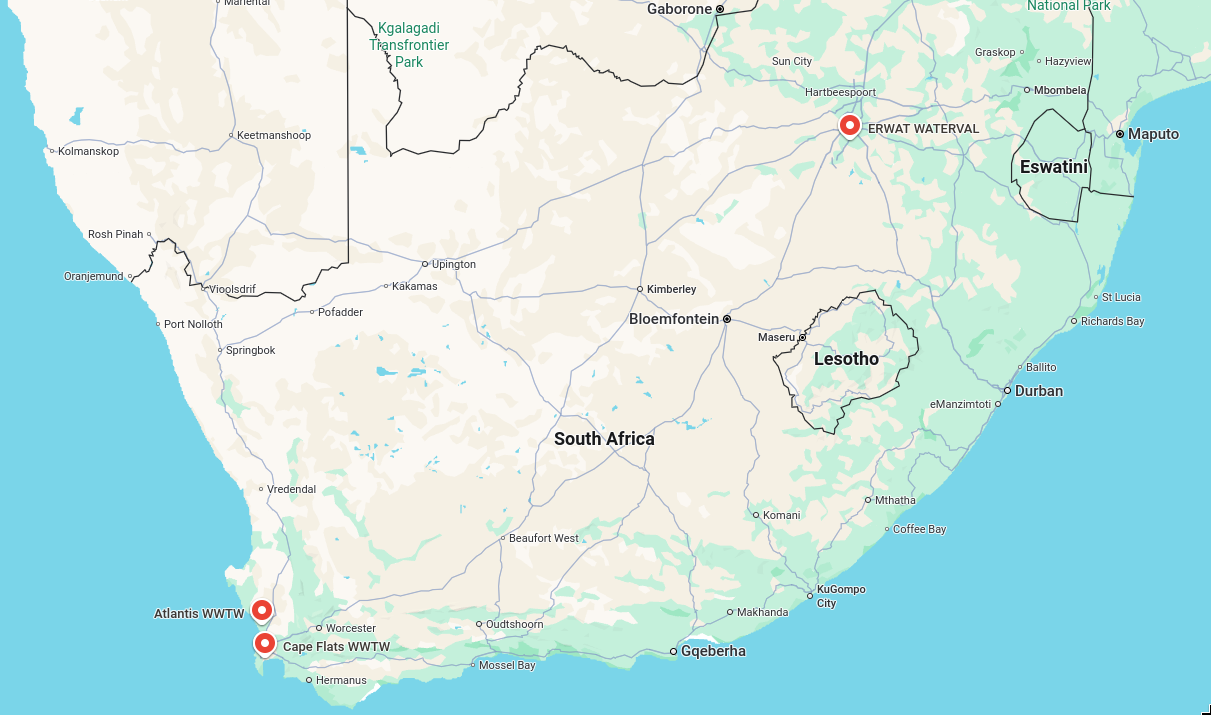
\includegraphics[width=0.6\textwidth]{figures/map.png} 
    \caption{Location of the five WWTW facilities in the dataset.}\label{fig:map} 
\end{figure}

\begin{figure}[htbp]
    \centering
    \begin{subfigure}[b]{0.32\textwidth}
        \centering
        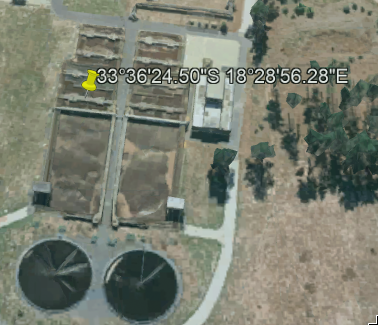
\includegraphics[width=\textwidth]{figures/atlantis_overview.png}
        \caption{Atlantis}\label{fig:atlantis_overview}
    \end{subfigure}
    \hfill
    \begin{subfigure}[b]{0.32\textwidth}
        \centering
        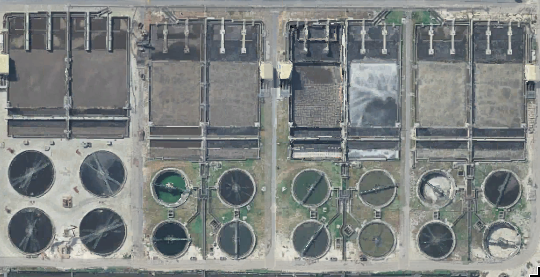
\includegraphics[width=\textwidth]{figures/capeflats_overview.png}
        \caption{Cape Flats}\label{fig:capeflats_overview}
    \end{subfigure}
    \hfill
    \begin{subfigure}[b]{0.3\textwidth}
        \centering
        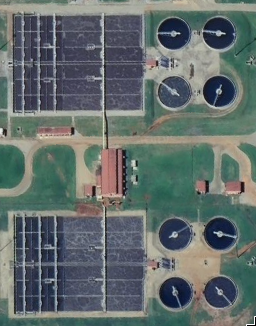
\includegraphics[width=\textwidth]{figures/waterval_overview.png}
        \caption{Waterval}\label{fig:waterval_overview}
    \end{subfigure}
    \hfill
    \begin{subfigure}[b]{0.3\textwidth}
        \centering
        \includegraphics[width=\textwidth]{figures/fisantekraal_overview.png}
        \caption{Fisantekraal}\label{fig:fisantekraal_overview}
    \end{subfigure}
    \hfill
    \begin{subfigure}[b]{0.3\textwidth}
        \centering
        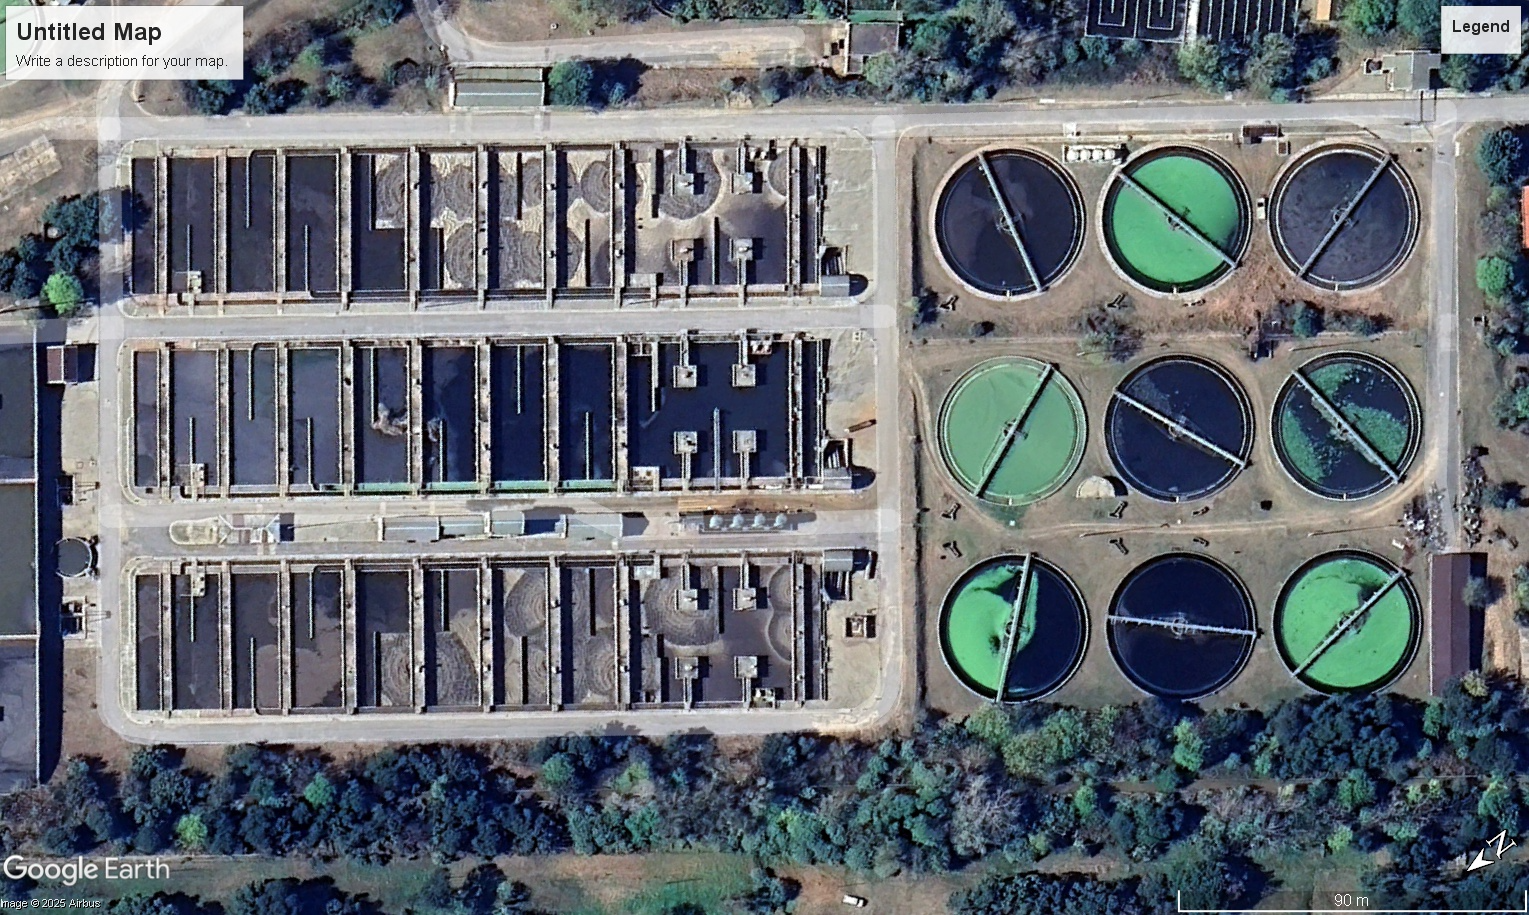
\includegraphics[width=\textwidth]{figures/noordelikewerke_overview.png}
        \caption{Noordelike Werke}\label{fig:noordelikewerke_overview}
    \end{subfigure}
    \caption{Overview of the Atlantis, Cape Flats, Waterval, Fisantekraal, and Noordelike Werke WWTW facilities.}\label{fig:facility_overviews}
\end{figure}

\section{Annotations}

Images were manually annotated using the VGG Image Annotator (VIA2) tool. Aerobic zones were labelled using rectangular bounding boxes, while clarifiers were labelled using circular regions, reflecting the physical shape of each structure. Each annotation carries a region attribute indicating the visible state of that component at the time the image was captured.

Aerobic zones were labelled into one of three categories, based on how much of the surface exhibits the characteristic "leopard print" aeration pattern. Examples are shown in Figure \ref{fig:aerobic_examples}:

\begin{itemize}
    \item \textbf{Functional}: the surface shows the leopard print pattern.
    \item \textbf{Suboptimal}: a third or more of the surface shows no leopard print, or the state is unclear.
    \item \textbf{Dysfunctional}: two thirds or more of the surface shows no leopard print, or is clearly dysfunctional.
\end{itemize}

Clarifiers were labelled into one of four categories, based on surface colour and visibility. Examples are shown in Figure \ref{fig:clarifier_examples}:

\begin{itemize}
    \item \textbf{Functional}: surface appears uniformly black.
    \item \textbf{Dysfunctional}: surface appears green.
    \item \textbf{Scum}: surface is not uniformly black.
    \item \textbf{Empty}: shadows are visible inside the tank.
\end{itemize}



Annotations are stored as VIA2 project files in JSON format. Each entry records the image filename, file size, and a list of regions, where each region specifies its shape (rectangle or circle), pixel coordinates, and the associated class label. An example entry for an aerobic zone annotation is shown below:

\begin{verbatim}
"Atlantis 01_2019.jpg3469910": {
  "filename": "Atlantis 01_2019.jpg",
  "size": 3469910,
  "regions": [
    {
      "shape_attributes": {
        "name": "rect",
        "x": 2707, "y": 931,
        "width": 2839, "height": 1381
      },
      "region_attributes": { "aerobic zone": "Dysfunctional" }
    }
  ],
  "file_attributes": {}
}
\end{verbatim}

Examples of the classes for aerobic zones and clarifiers are shown in Figures \ref{fig:aerobic_examples} and \ref{fig:clarifier_examples} respectively.

\begin{figure}[htbp]
    \centering 
    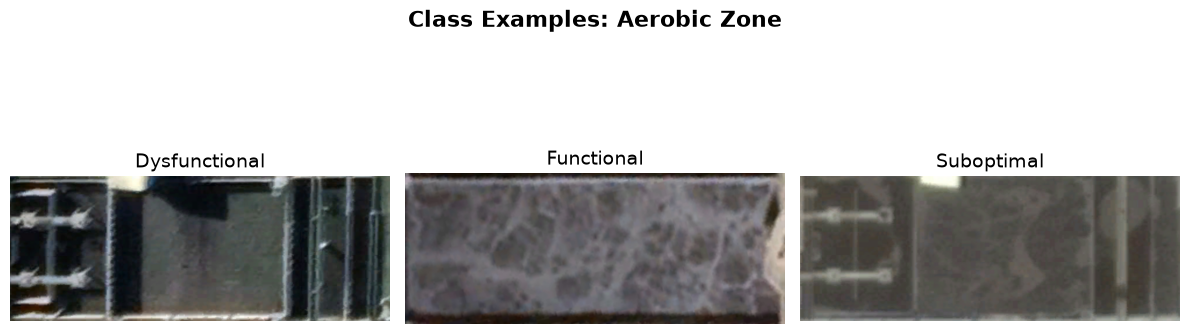
\includegraphics[width=0.75\textwidth]{figures/aerobic_examples.png} 
    \caption{Examples of aerobic zone classes.}\label{fig:aerobic_examples}
\end{figure}

\begin{figure}[htbp]
    \centering 
    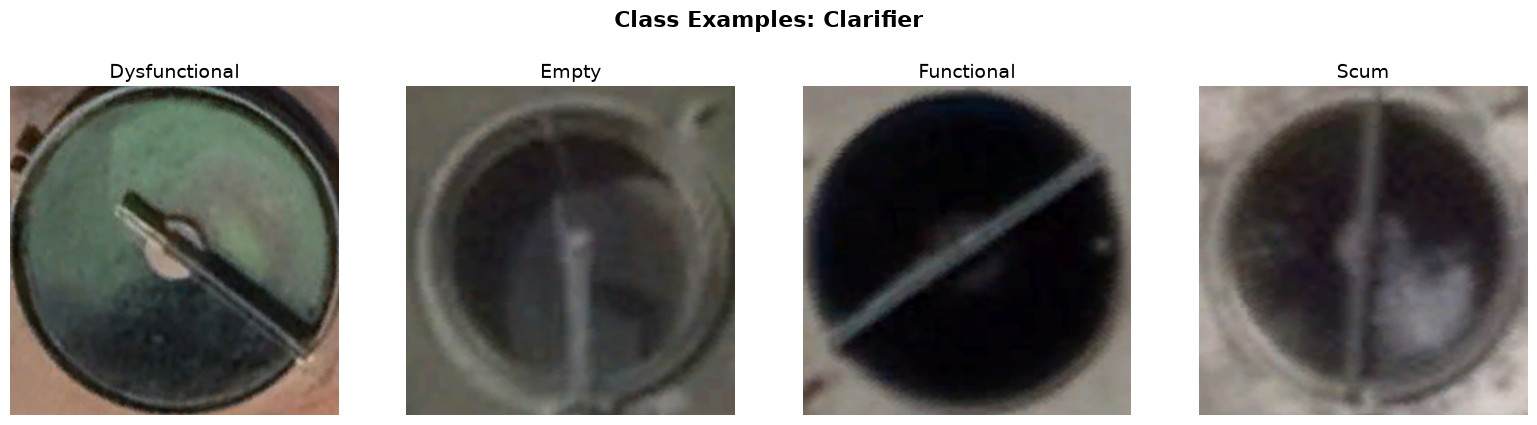
\includegraphics[width=0.75\textwidth]{figures/clarifier_examples.png} 
    \caption{Examples of clarifier classes.}\label{fig:clarifier_examples}
\end{figure}

\section{Facility Structure}

The three facilities differ slightly in how their data is organised, reflecting differences in plant layout.

\textbf{Atlantis} consists of a single biological reactor, so its 48 images are stored in one folder with no subdivisions. Aerobic zone and clarifier labels are each stored in a single JSON file.

\textbf{Cape Flats} consists of four separate reactor units (CF1–CF4), each with its own image folder and containing between 92 and 100 images. Each unit has its own aerobic zone and clarifier label file.

\textbf{Waterval} consists of two reactor units, referred to as Top and Bottom, with 37 and 36 images respectively. Each unit has its own aerobic zone and clarifier label file.

\textbf{Fisantekraal} consists of a single reactor unit, with 63 images stored in one folder. Only clarifiers have been labeled and stored in a single JSON file.

\textbf{Noordelike werke} consists of a single reactor unit, with 45 images stored in one folder. Only clarifiers have been labeled and stored in a single JSON file.

Table~\ref{tab:dataset_summary} summarises the structure of the dataset across the three facilities.

\begin{table}[h]
\centering
\caption{Summary of the dataset by facility}\label{tab:dataset_summary}
\begin{tabular}{lccc}
\toprule
\textbf{Facility} & \textbf{Units} & \textbf{Images} \\
\midrule
Atlantis   & 1 & 48                 \\
Cape Flats & 4 & 382 (96+94+92+100) \\
Waterval   & 2 & 73 (37+36)         \\
Fisantekraal   & 1 & 63                 \\
Noordelike werke   & 1 & 45                 \\
\bottomrule
\end{tabular}
\end{table}

This structural difference between facilities — a single unit at Atlantis, four at Cape Flats, and two at Waterval — is factored into the data pipeline described in Section~\ref{sec:pipeline}, since each facility's images and labels need to be parsed slightly differently before they can be fed into the CNN.


\section{Data Preparation}\label{sec:pipeline}

Before the labelled regions can be used to train a classifier, they need to be extracted from the full facility images and organised by class. This is handled by a preparation script (\texttt{prep.py}), which reads the VIA2 annotation files, crops out each labelled region, and saves the crops into a folder structure that can be loaded directly with \texttt{torchvision.datasets.ImageFolder}.

The script processes each facility one unit at a time, since Atlantis, Cape Flats, and Waterval each have a different number of units and label files. For every unit, it opens the aerobic zone and clarifier JSON files separately and works through each image entry in turn.

For each labelled region in an image, the script performs the following steps:

\begin{itemize}
    \item Reads the shape attributes of the region. Aerobic zones are stored as rectangles, defined by an x and y coordinate along with a width and height. Clarifiers are stored as circles, defined by a centre point and a radius.
    \item Converts the shape into a bounding box that can be used to crop the image, since Python's Image Library crop function requires a rectangular box even for the circular clarifier regions.
    \item Clamps the box to the edges of the image, in case a region was drawn slightly outside the image bounds during annotation.
    \item Reads the class label from the region attributes and checks it against the expected set of classes for that component. Labels are also normalised, so that small inconsistencies in capitalisation from the manual annotation process do not create extra classes.
    \item Crops the region out of the source image and saves it as a JPG file inside the folder matching its class label.
\end{itemize}

Each output filename encodes the facility, unit, and original image name, so that a crop can always be traced back to the source image it came from. For example, a crop from unit CF2 at Cape Flats would be saved with a filename beginning \texttt{CapeFlats\_Images-CF2\_...}, followed by the original image name and a region number.

The result is a folder structure with one top-level folder per component and one subfolder per class:

\begin{verbatim}
cnn_dataset/
    aerobic_zone/
        Functional/
        Suboptimal/
        Dysfunctional/
        Empty/
    clarifier/
        Functional/
        Dysfunctional/
        Scum/
        Empty/
        Stagnant/
\end{verbatim}

This structure means the aerobic zone and clarifier sub-images are treated as two separate classification problems, each with its own set of class folders, rather than a single combined dataset.


\section{Excluded from the dataset}
During processing, two annotated classes were found to have too few examples to be usable for training. The aerobic zone dataset contained a single region labelled \textbf{Empty}, and the clarifier dataset contained four regions labelled \textbf{Stagnant}. Both classes were therefore excluded from the final dataset, and the corresponding regions were not cropped or saved. A class with only one or a handful of examples cannot be meaningfully split into training, validation, and test sets, and would not give the CNN enough examples to learn a reliable representation of that class. Including such a small class also risks skewing the overall class balance and encouraging the model to simply ignore it during training, since the loss contribution from so few examples is negligible compared to the other classes. The excluded regions were still counted separately by the preparation script, so their presence in the original annotations is not lost, but they play no further part in the classification task.


\section{Data Splitting}

\subsection{Leave-one-out Split}

To evaluate how well the trained classifier generalises to WWTW facilities it has never encountered, the dataset was partitioned using a leave-one-out strategy rather than a random split. One facility, chosen from the five available (Atlantis, Cape Flats, Waterval, Fisantekraal, and Noordelike werke), was the test facility and withheld from training entirely: none of its images appear in the training or validation sets, and it plays no part in model selection or hyperparameter tuning. Note that this is repeated five times, once for each facility. This guarantees that test performance reflects the model's ability to classify components at an unseen site.

This split was applied independently for each facility component, aerobic zone and clarifier, since the two have different classes and different image sets.

Once the test facility was removed, the remaining four facilities' images were divided into training and validation sets. A random split at this stage risks an uneven mix: validation could end up dominated by whichever facility or unit happened to contribute the most images, or by images from a narrow range of capture dates, which would give an unrepresentative estimate of validation performance.

To avoid this, images were first grouped by facility, unit and class (some facilities have more than one unit, for example Cape Flats has 4 units each with its own set of images). Different units at the same facility can differ in lighting, or capture date, so treating them as separate groups during shuffling keeps that variation spread across both training and validation rather than concentrated in one. Within each group, images were shuffled using a fixed random seed to mix capture dates before being partitioned according to a fixed validation ratio (20\%). Splitting within these smaller groups rather
than across the whole set ensures that every facility, unit, and class combination among the four training facilities is represented in both
the training and validation sets, in proportion to how much data it contributes. An example is shown in Figure \ref{fig:leave_one_out approach} of the Waterval facility being withheld as the test set.

\begin{figure}[h]
    \centering
    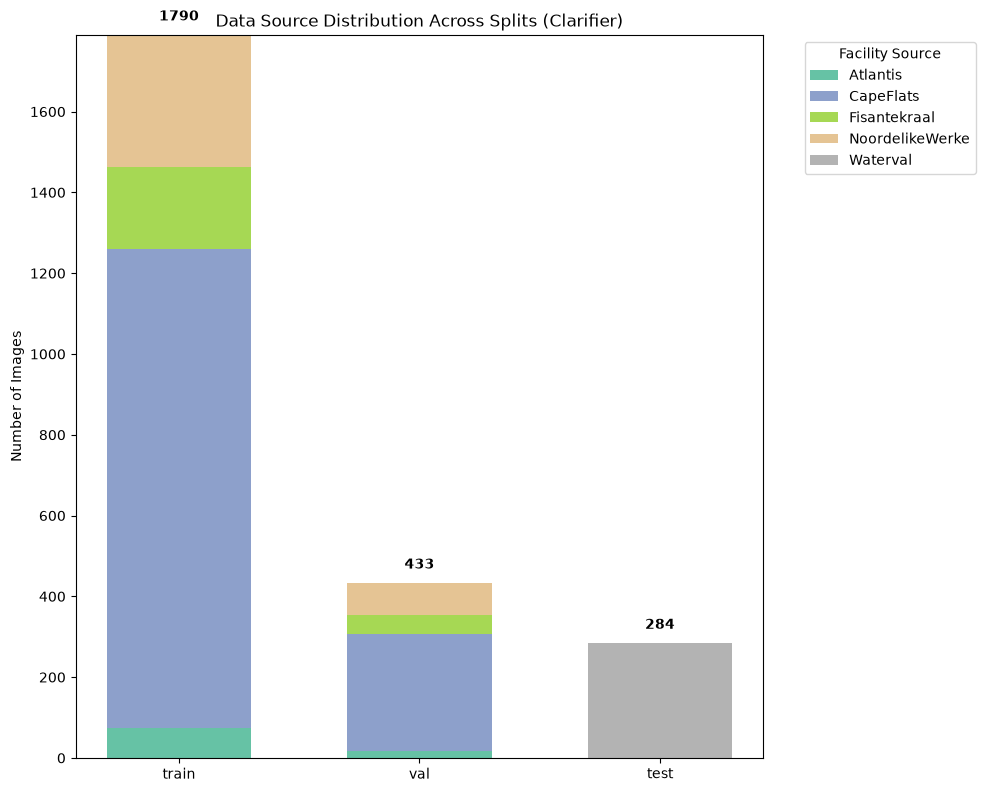
\includegraphics[width=0.7\textwidth]{figures/leave_one_out.png} 
    \caption{Illustration of the leave-one-facility-out split. The test facility is withheld from training and validation, while the remaining four facilities are split into training and validation sets.}
    \label{fig:leave_one_out approach}
\end{figure}

\subsection{Stratified Train/Validation Split}
Before adopting the leave-one-out approach described above, a stratified split was used to produce training, validation, and test
sets directly from the dataset, without holding any facility out. This split follows a 70/20/10 training/validation/test ratio and uses the same facility, unit, class grouping and shuffling procedure: images within each group are shuffled under a fixed random seed before being partitioned, so that every facility, unit, and class combination is represented across all three sets in proportion to how much data it contributes, and no single facility or unit dominates any one split.

\section{Relabeling}

To improve label quality, a relabeling notebook was built using Jupyter widgets to review the clarifier dataset in full and correct labels where
necessary. Every clarifier image was reviewed manually, rather than looking at what the classifier got wrong which could potentially introduce bias. For each image, the notebook displays the image alongside its current label and a row of per-class buttons; clicking a button records the corrected label without requiring any manual file editing. Corrections are written to a separate \texttt{relabel/} working copy of the annotation files rather than overwriting the originals, so the original VIA2 labels remain intact and every correction can be traced back to what it changed.

Figure \ref{fig:relabel_example} shows a case, where an image originally labelled ``Scum'' was corrected to ``Empty'' after review, since the dark
region was identified as shadow rather than surface scum. Figure \ref{fig:relabel_process_example} shows the review interface itself, with the original label displayed in yellow next to the image and the correction buttons below it.

\begin{figure}[h]
\centering
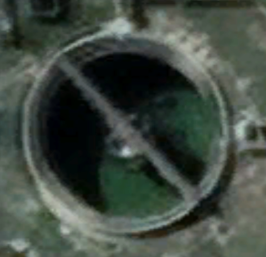
\includegraphics[width=0.2\textwidth]{figures/relabel_example.png}
\caption{An incorrectly labelled clarifier. The original label was ``Scum,''
but the correct label is ``Empty,'' since the dark region is a shadow rather
than surface scum.}
\label{fig:relabel_example}
\end{figure}

\begin{figure}[h]
\centering
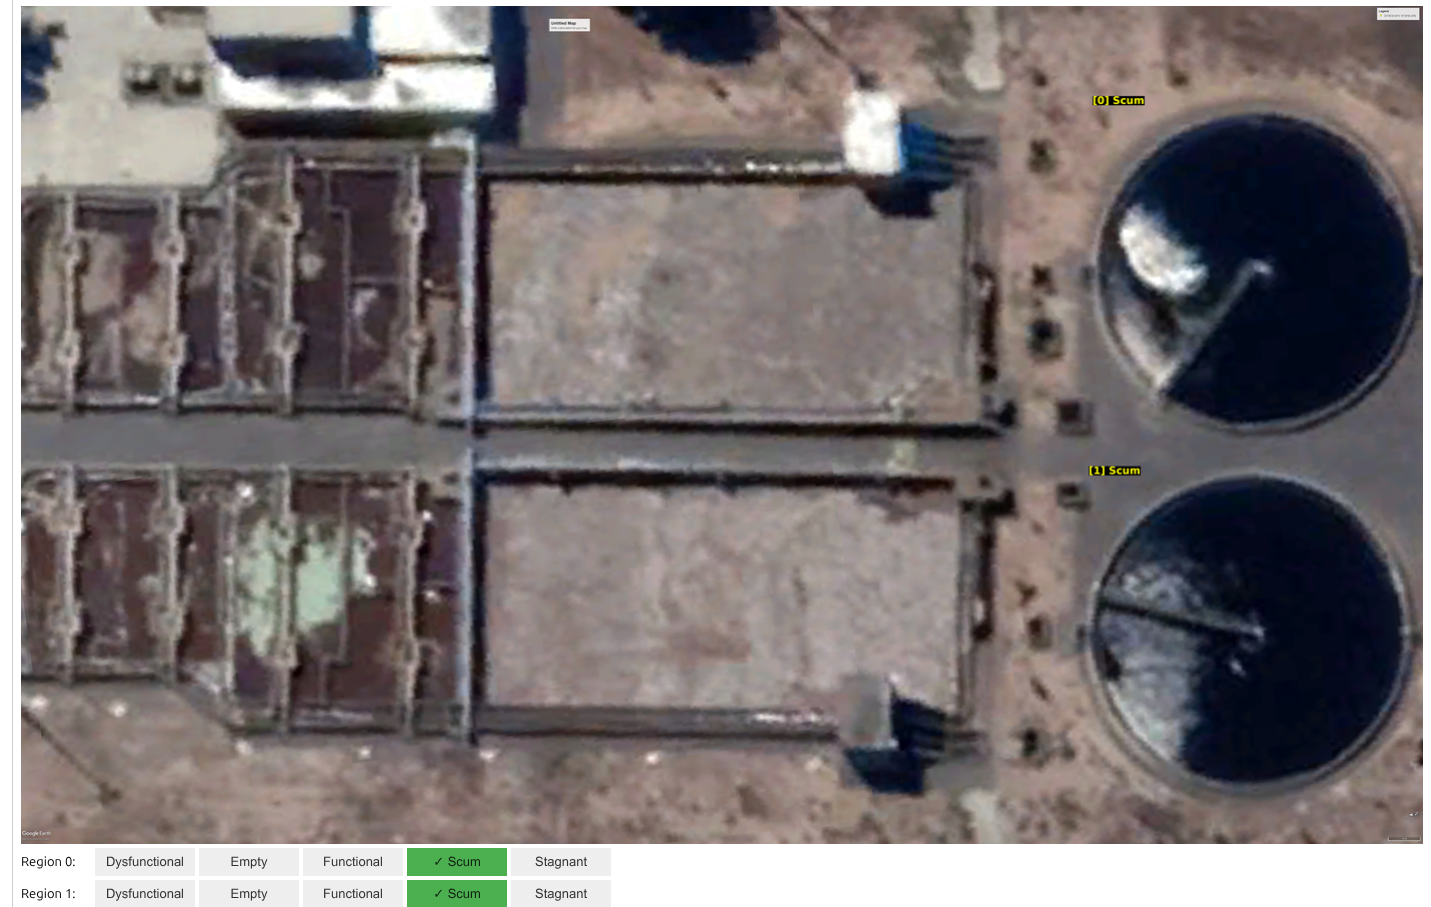
\includegraphics[width=0.7\textwidth]{figures/relabel_process_example.png}
\caption{The relabeling interface, showing the original label and the
per-class correction buttons.}
\label{fig:relabel_process_example}
\end{figure}

\section{Summary Table}
\begin{table}[htbp]
    \centering
    \caption{Summary of image counts per class for the Aerobic Zones.}
    \label{tab:aerobic_summary}
    \begin{tabular}{l rrr}
        \toprule
        \textbf{Facility} & \textbf{Dysfunctional} & \textbf{Functional} & \textbf{Suboptimal} \\
        \midrule
        Atlantis         & 14  & 58  & 19  \\
        Cape Flats 1     & 113 & 44  & 37  \\
        Cape Flats 2     & 146 & 21  & 21  \\
        Cape Flats 3     & 137 & 15  & 32  \\
        Cape Flats 4     & 166 & 12  & 22  \\
        Waterval Top     & 85  & 344 & 15  \\
        Waterval Bottom  & 144 & 199 & 77  \\
        Fisantekraal     & 0   & 0   & 0   \\
        Northern Works   & 0   & 0   & 0   \\
        \midrule
        \textbf{TOTAL}   & \textbf{805} & \textbf{693} & \textbf{223} \\
        \bottomrule
    \end{tabular}


    Note that Fisantekraal and Northern Works do not have any aerobic zones labelled.
    
    \vspace{2.5em} 
    
    \caption{Summary of image counts per class for the Clarifiers.}
    \label{tab:clarifier_summary}
    \begin{tabular}{l rrrr}
        \toprule
        \textbf{Facility} & \textbf{Dysfunctional} & \textbf{Empty} & \textbf{Functional} & \textbf{Scum} \\
        \midrule
        Atlantis         & 0   & 2   & 36   & 52  \\
        Cape Flats 1     & 31  & 60  & 177  & 76  \\
        Cape Flats 2     & 60  & 33  & 181  & 90  \\
        Cape Flats 3     & 19  & 19  & 209  & 121 \\
        Cape Flats 4     & 41  & 1   & 129  & 229 \\
        Waterval Top     & 71  & 0   & 69   & 0   \\
        Waterval Bottom  & 7   & 0   & 26   & 111 \\
        Fisantekraal     & 19  & 9   & 106  & 118 \\
        Northern Works   & 127 & 13  & 113  & 152 \\
        \midrule
        \textbf{TOTAL}   & \textbf{375} & \textbf{137} & \textbf{1046} & \textbf{949} \\
        \bottomrule
    \end{tabular}
\end{table}